%%%%%%%%%%%%%%%%%%%%%%%%%%%%%%%%%%%%%%%%%
% University/School Laboratory Report
% LaTeX Template
% Version 3.1 (25/3/14)
%
% This template has been downloaded from:
% http://www.LaTeXTemplates.com
%
% Original author:
% Linux and Unix Users Group at Virginia Tech Wiki 
% (https://vtluug.org/wiki/Example_LaTeX_chem_lab_report)
%
% License:
% CC BY-NC-SA 3.0 (http://creativecommons.org/licenses/by-nc-sa/3.0/)
%
%%%%%%%%%%%%%%%%%%%%%%%%%%%%%%%%%%%%%%%%%

%----------------------------------------------------------------------------------------
%	PACKAGES AND DOCUMENT CONFIGURATIONS
%----------------------------------------------------------------------------------------

\documentclass{article}

\usepackage[version=3]{mhchem} % Package for chemical equation typesetting
\usepackage{siunitx} % Provides the \SI{}{} and \si{} command for typesetting SI units
\usepackage{graphicx} % Required for the inclusion of images
\graphicspath{ {./img/} }
\usepackage[numbers]{natbib} % Required to change bibliography style to APA
\usepackage{amsmath} % Required for some math elements 
\usepackage{listings}
\usepackage{xcolor}
\usepackage[legalpaper, portrait, margin=2.5cm]{geometry}
\usepackage[hidelinks]{hyperref}
\usepackage{siunitx}

\definecolor{mGreen}{rgb}{0,0.6,0}
\definecolor{mGray}{rgb}{0.5,0.5,0.5}
\definecolor{mPurple}{rgb}{0.58,0,0.82}
\definecolor{backgroundColour}{rgb}{0.95,0.95,0.92}

\lstdefinestyle{CStyle}{
	backgroundcolor=\color{backgroundColour},   
	commentstyle=\color{mGreen},
	keywordstyle=\color{magenta},
	numberstyle=\tiny\color{mGray},
	stringstyle=\color{mPurple},
	basicstyle=\footnotesize,
	breakatwhitespace=false,         
	breaklines=true,                 
	captionpos=b,                    
	keepspaces=true,                 
	numbers=left,                    
	numbersep=5pt,                  
	showspaces=false,                
	showstringspaces=false,
	showtabs=false,                  
	tabsize=2,
	language=C
}


\lstset { %
	language=C++,
	backgroundcolor=\color{black!5}, % set backgroundcolor
	basicstyle=\footnotesize,% basic font setting
}


\setlength\parindent{0pt} % Removes all indentation from paragraphs

\renewcommand{\labelenumi}{\alph{enumi}.} % Make numbering in the enumerate environment by letter rather than number (e.g. section 6)

%\usepackage{times} % Uncomment to use the Times New Roman font

%----------------------------------------------------------------------------------------
%	DOCUMENT INFORMATION
%----------------------------------------------------------------------------------------

\begin{document}

\begin{titlepage}
	\begin{center}
		\vspace*{1cm}
		
		\Huge
		\textbf{PROJECT REPORT}
		
		\vspace{0.5cm}
		\LARGE
		W11GROUP09
		
		\vspace{1.5cm}
		
		\textbf{Authors}
		\begin{tabular}{l r}
			% Date the experiment was performed
			& Victor Chu 480080303 \\ & Keene Hoang 470020243 \\ & Lucian Nguyen 470051328
			% Instructor/supervisor
		\end{tabular}
		\vspace{1.8cm}
		
		The Maze Escaper\\
		%Blablabla
		\vspace{2cm}
		
\includegraphics[width=\linewidth]{usyd-logo.jpg}
		\vspace{0.8cm}
		\date{\today} % Date for the report
		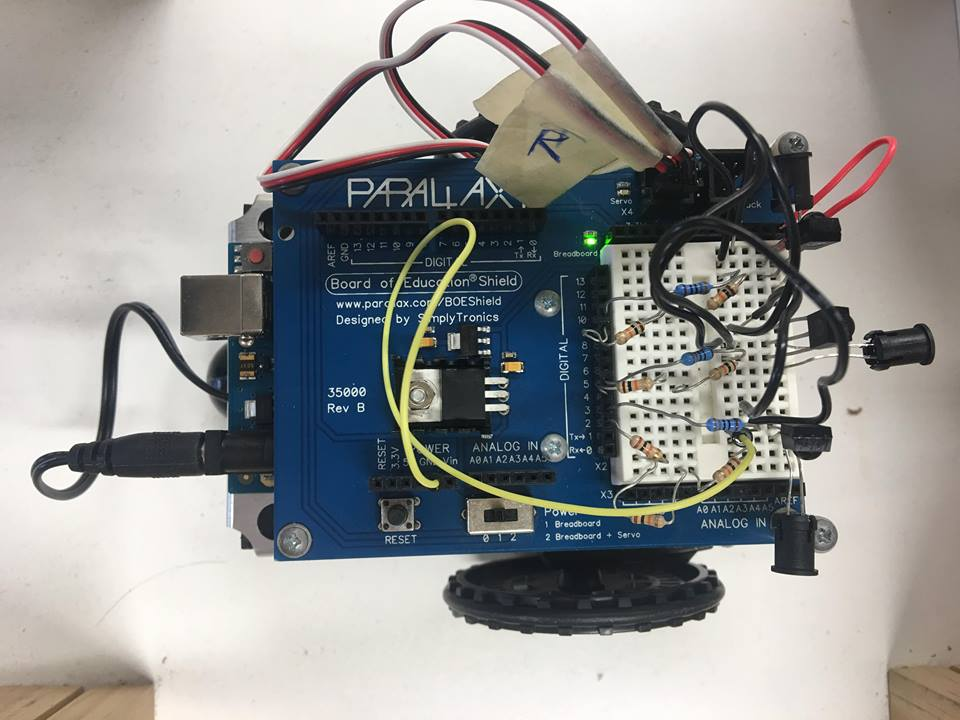
\includegraphics[width=400pt]{pic5.jpg}

		
		
	\end{center}
\end{titlepage}
\tableofcontents
\newpage

%section1
\section{Introduction}

\subsection{The problem and motivation}
Imagine one day, you are in a maze game, one way in and one way out only, its complexity of the maze will irritate you, and you will feel lost. Maze game is not just a game, it is a fundamental problem of the navigation system and finding the path and even the shortest part is a hard and crucial mission. However, the solution is simple and executable. The "Maze Escaper" is a robot which can solve simple mazes (with up to 3 directions for each fork). Nonetheless, the speed of solving the problem is another problematic problem because today the speed of performance in navigation systems becomes more and more critical. From that difficulties, they are the motivation for the team to work out the elegant solution and the robot can solve the maze in the shortest possible time.\\

\subsection{Previous work on maze solving problem}
There are two most straightforward and well-known algorithms for solving maze:
\subsubsection{Random mouse algorithm}
This is the most straightforward and most insufficient algorithm. Every time the robot reaches an intersection, it randomly chooses the direction. If it reaches to the point where it cannot go anywhere, it turns back and does the same way to find the way out \cite{ref1}. This algorithm consumes a very long time to solve a maze because of its inconsistency.\\

\subsubsection{Wall follower algorithm}
This is also a simple algorithm. The robot only needs to keep stick with the left or right wall \cite{ref1}. However, the weakness of this algorithm is that there will be cases where the robot move around forever and never find the destination.\\

\subsubsection{Depth-first search algorithm - one of the best maze-solving algorithm} 
The two previous algorithms show obvious weaknesses in term of time and efficiency. The depth-first search algorithm is born to solve those remaining problems. It only finds the new ways and never repeat the old route which saves much time to solve the maze.\\

\begin{figure}[h!]
	\centering
		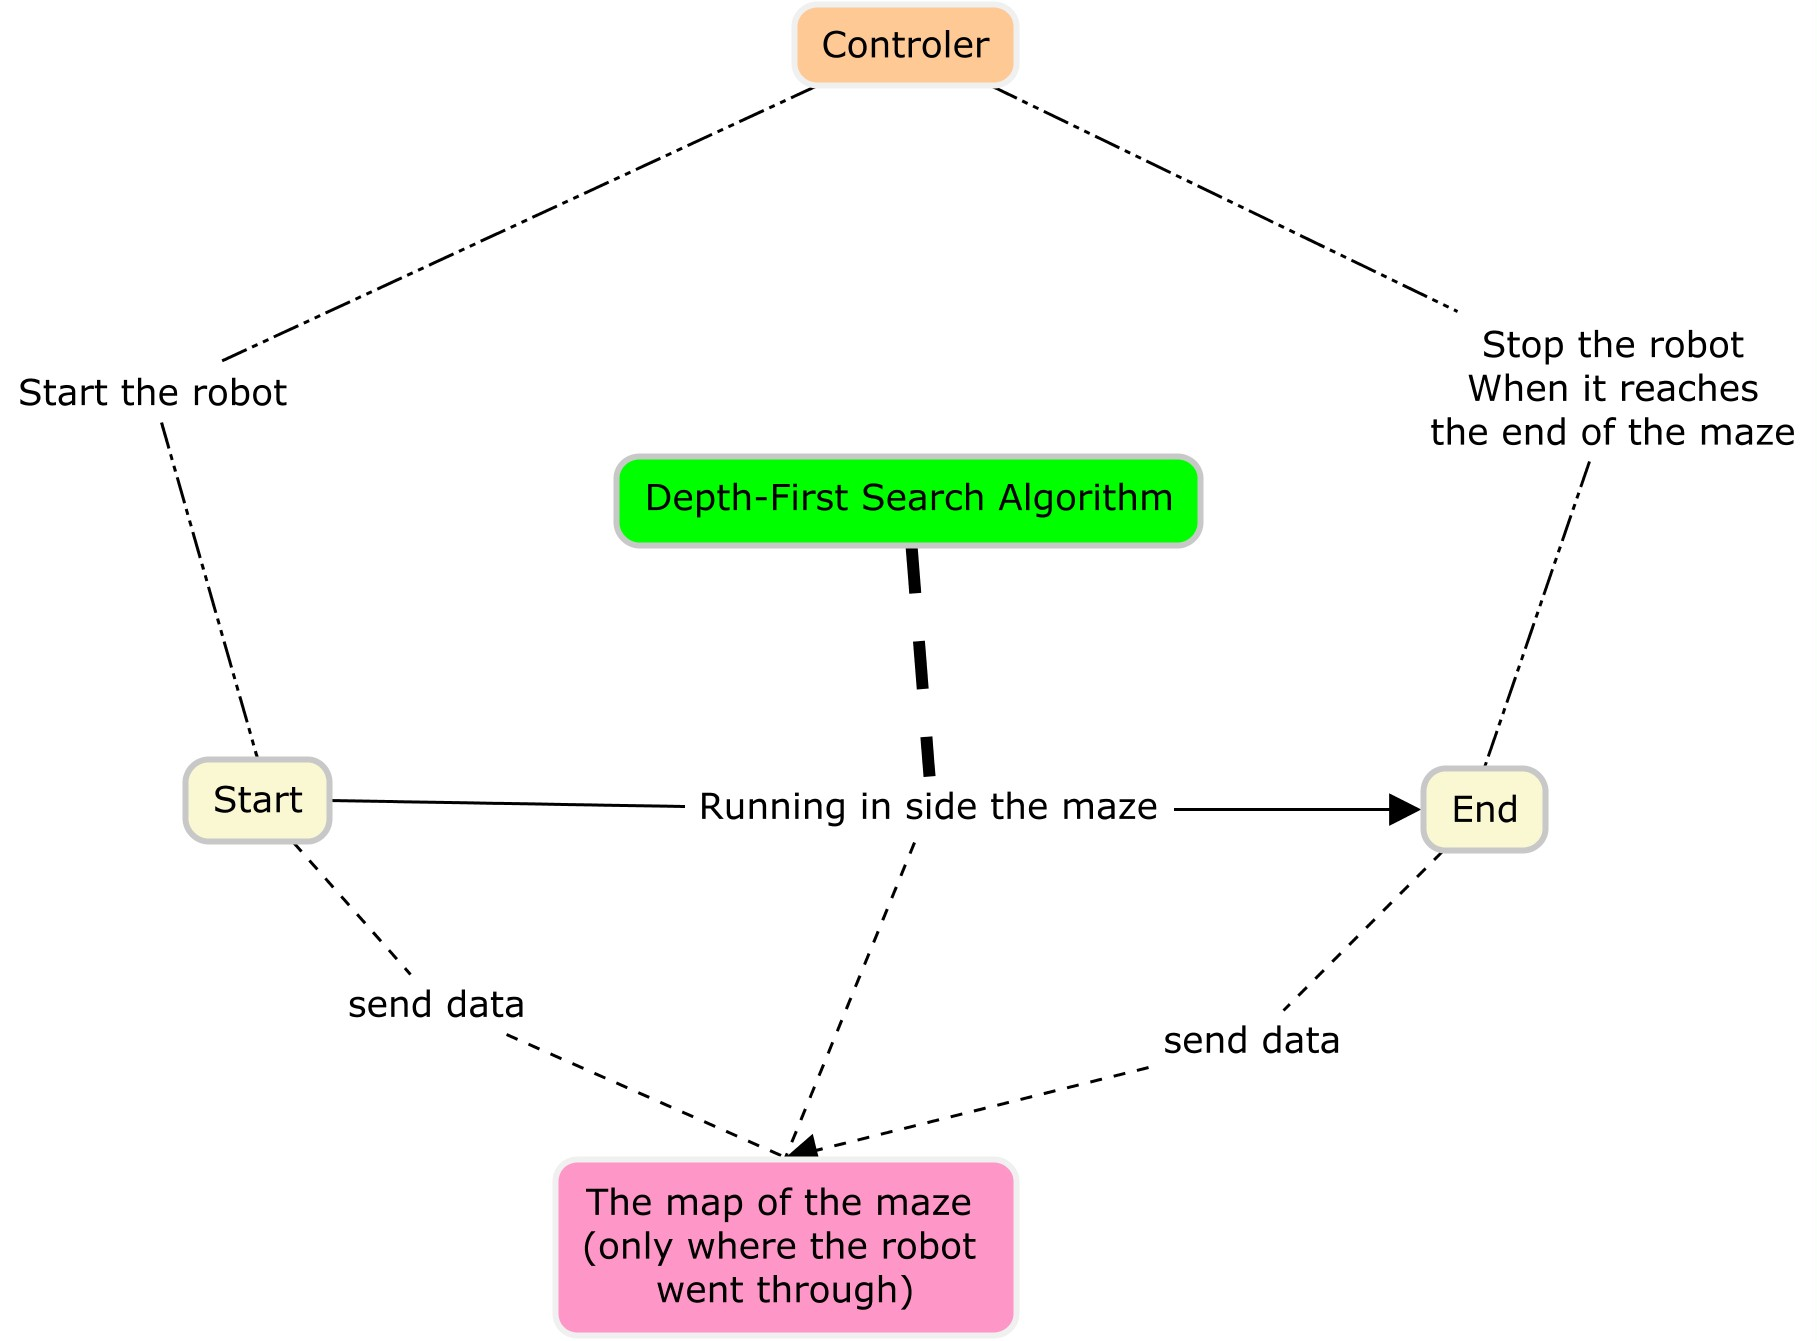
\includegraphics[width=\linewidth]{pic3.jpg}
	\caption{Depth-First Search Algorithm (Sketched by Lucian)}
	
\end{figure}

\subsubsection{The final choice of algorithm}
After considering those algorithms regarding complexity and efficiency, Wall follower algorithm is chosen. Also, after the project, this algorithm will be upgraded to solve loop maze situation.\\

\subsection{Hypothesis}
The robot is only solved for the simple mazes without any loops. Additionally, it stops when the controller gives a stop command manually. The reason is that we want to apply Blue-tooth to make interaction with the robot.

\subsection{Objectives}
\begin{itemize}
	\item To build the simple robot using sensors, output devices and Bluetooth communication
	\item To understand the importance of time, teamwork and leadership
	\item To solve the real-life problem by applying Arduino
	\item To code fluently and deal with bugs or errors
	\item To access the concept of project management
	\item To use fluently external website and software to write the report, draw sketches, manage the project and vice versa
\end{itemize}

 
%----------------------------------------------------------------------------------------
%	SECTION 2
%----------------------------------------------------------------------------------------
\newpage
\section{Description of the product}
\subsection{Part lists}
\begin{tabular}{ll}
The Boe-Bot Robotic Shield & {1}\\
Arduino board & {1}\\
110-Ohm resistors & {3}\\
10K-Ohm resistors & {7}\\
IR receivers & {3}\\
IR LEDs & {3}\\
Long jumper wires & {1}\\
Short jumper wires & {7}\\
Blue-tooth shields & {2}\\



\end{tabular}

%----------------------------------------------------------------------------------------
%	SECTION 3
%----------------------------------------------------------------------------------------
\newpage
\section{Project processes}

\subsection{Team routine, robot assembly and first program}
Before the lab session, the team listened to the tutor's instruction about essential information of the project regarding project management, marking criteria, team member's principle, project processes, deadline and so on.\\
\subsubsection{Be familiar with Trello for project management}
Trello is the project management application used by the team in the project with tutor's supervision. \\
Members of the team can create and customise the tasks and contents while the project is running.\\
The team W11GROUP09 Trello's roster:
\begin{itemize}
	\item Lucian: facilitator, reporter 
	\item Keen: issue tracker, reporter
	\item Thang: issue tracker, idea curator
\end{itemize}

\subsubsection{CMapTools' knowledge}
The goal of this exercise is becoming acquainted with CMapTools, software which helps to design quite quickly some ideas with concepts (squares) as well as relations (edges). The reporter makes use of this software to capture the way the project plan evolves from Week 8 to Week 12. In Week 8 the team is going to produce the first model of the project concept, and every week there'll be an evolution of the thought that is uploaded on the project management tool - Trello.


\subsubsection{Boe-Bot assembly}
The Boe-Bot is assembled formerly, but the team still needs to read  \href{https://canvas.sydney.edu.au/courses/5511/pages/Boe-Bot%20assembly?titleize=0}{\textit{the given document}} to know how to build circuits and also connect servos to the Arduino.
	
\subsubsection{Servo Motor and BOE Shield-Bot Navigation}
After completing the exercise, the team oughts to be ready to reply to the following questions:
\begin{itemize}
	\item What's a servo motor?
	\item How can I create the robot to move forward, overturn, switch left/right?
	\item How can I manage the movement speed?
\end{itemize} 

\subsubsection{Tactile Navigation with Whiskers}
After solving these exercises, the team must be ready to reply to the following questions:
\begin{itemize}
	\item How does BOE Shield-Bot sense its surrounding through the whiskers?
	\item How can I make the robot stay away from obstacles?
\end{itemize} 

\subsection{Robot Vision, Communication and Brain Storming}

\subsubsection{Prepare Brainstorming Session}
\begin{itemize}
	\item Browse the two papers of \href{https://canvas.sydney.edu.au/courses/5511/files/2801346/download?wrap=1}{\textit{Brainstorm Rules}} and \href{https://canvas.sydney.edu.au/courses/5511/files/2801350/download?wrap=1}{Facilitate a Brainstorm} offered as resources.
	\item Jot on the 2 or maybe three rules that summarise just how a brainstorming session functions.
\end{itemize} 

\subsubsection{Robot Vision}
\begin{itemize}
    \item \textbf{IR assembly and testing}: After constructing the IR LEDs and receivers, the team switch 220 \si{\ohm} and 2000 \si{\ohm} to 390 \si{\ohm} and 4700 \si{\ohm} respectively. We see that when we increase the value of a resistor, the sensitivity of IR receivers decreases as well as the strength of IR LEDs. Finally, Test the right and left receiver and LEDs.
    \item \textbf{Using IR as eyes}: IR LEDs and receivers are employed to identify obstacles the same as the whiskers, but they are more sensitive and space-saving.
    \item \textbf{Detection range}: Since the strength of IR light reduces over distance, the detection of IR reflected off of a wall depends on its emission power. Thus, greater emission energy is going to allow the IR light to go the farther distance but still have the power that is enough to be recognised by the receivers. We examine the emission energy as well as distance connection. The optimum detection distance provided LED resistance of 47K \si{\ohm}, 10K\si{\ohm}, 4700 \si{\ohm}, 1000 \si{\ohm}, 470 \si{\ohm} is 3.3cm, 4.5cm, 5.3cm, 9.1cm, 12.3cm respectively.
    \item \textbf{Drop-off detector} In the same way the IR LEDs and receivers could be utilised to identify a hole or perhaps gap on the robot 's path.
\end{itemize} 

\subsubsection{Brainstorming Session}
\begin{itemize}
	\item Agree together with teammates around the length of the brainstorm session (15 minutes).
	\item Prepare A4 papers and pens to take notes and draw.
	\item Take an active posture, get close together.
	\item Shoot all of the ideas that come from the conference. Our initial idea is a robot which can move around a terrain controlled by an accelerometer. However, this idea is too simple and not creative enough for us. Then, Lucian has come up with the idea of making a robot can solve a simple maze using some algorithms.
\end{itemize}


\subsubsection{Serial Communication via Bluetooth}
Programming Bluetooth interaction in Arduino requires to perform one system in a single Arduino board to manage an additional circuit that has the Bluetooth antenna and added circuitry. Through 2 pins is communicated by these two systems. A second system is performing in the next method to manage the next Bluetooth antenna along with added circuitry. This implies that you are going to have to deal with two systems within the same IDE to publish to 2 boards attached to 2 various ports.


\subsection{Design Sketch and Phase 1 Implementation}
\subsubsection{Prepare Sketch of the Prototype of your Project
}

\begin{itemize}
    \item Create one explanation of the possible \textbf{real product} to distribute to the concern of the teammates with a specific description. The following paragraph is written by a member of the team - Keene:\\
    \textit{``Firstly, I want to address the mechanism of the robot regardless of applicational areas, which is exploring and mapping its surrounding. Imagine this maze-solving robot is applied in a real-life situation, especially in sketching out areas unbeknownst to us, for instance, abandoned areas post-war. There might be difficulties in distinguishing between a wall and other issues such as a big stone, which can be compensated with an upgrade in the detection of size. Therefore, depending on the results, the robot could decide if the obstacle is a wall or small barriers that it can overcome. Having explained the feature of detecting blockage and mapping required areas, let’s talk about its possible contribution in the Medical field. More specifically, our robotic features can be equipped onto nanorobots before being released into the circulatory system. Subsequently, we could use these nanorobots to treat dyslipidaemia, a disease that results in an abnormal amount of lipids in the blood. This is very promising considering nanorobots are capable of detecting the position and magnitude of lipid then collect critical data for the people involved. Experts can use the data to prescribe suitable medication for patients whose awareness hopefully, are raised about their conditions. Apart from that, Nano Surgery also shows prospect as the surgical approach to curing dyslipidaemia diseases.``}
	\item Project Team Meeting outside the lab within 1 hour.
\end{itemize}

\subsubsection{First Implementation Phase}
In the first implementation phase, activities are:
\begin{itemize}
	\item Check if the availability of components by building a simple board. Also, all the components are good to go.
	\item Attach sensors, IR LEDs, and jump wires. The number of components is high that makes us hard to attach due to lack of space.
	\item Adjust the resistors for IR sensors and LEDs to detect the wall in the required distance. This activity costs the team a significant amount of time.
	\item Check the detection of left, middle, and right sensors by Serial printing the value of all states. The team successfully finish phase 1 of the implementation stage.
\end{itemize}

\subsubsection{Write brief session report}
Lucian is in charge of doing it during and after the lab.

\subsection{Implementation Phase}

\subsubsection{Second Implementation Phase}
\begin{itemize}
    \item Change the input pin of the right IR LED and sensor from pins 0, one into pins 2, 3. Because pins 0 and one are used for serial communication.
    \item Test Bluetooth shields by sending the state from Slave to Master. We have a problem with reading the information from Slave shields. The info comes into the Master is delayed and cannot be detected. Therefore, we run out of time to adjust.
\end{itemize}

\subsubsection{Write brief session report}
Lucian is in charge of doing it during and after the lab.

\subsection{Implementation and Initial Testing}
\subsubsection{Finish Implementation and Initial Testing}
\begin{itemize}
	\item We find out the right way to read the output of the Slave by using \textit{BluetoothSerial.print()} and \textit{BluetoothSerial.read()}.
	\item The detection of IR sensors are corrupted again that causes us to switch the resistors many times.
	\item First runs the robot in the most straightforward cases: U-shape maze and only-turning-left maze.
\end{itemize}
\subsubsection{Write brief session report}
Lucian is in charge of doing it during and after the lab.

\subsection{Implementation and Final Testing}
We have to change the algorithm because the use of a stack is not efficient. The robot cannot traverse the path as expected.\\
The initial algorithm is a Depth-First Search algorithm which has turned into Left-hand Wall Following algorithm.\\
The sensors have problems again because the electric connection of the left corner of the BOE board is shut down (probably we forgot to take the batteries off at the end of the previous lab). Then we change the brand new BOE Bot and attach all components again.
%----------------------------------------------------------------------------------------
%	SECTION 4
%----------------------------------------------------------------------------------------
\newpage
\section{Implementation}
\subsection{Left-hand rule}
For this particular presentation, the bot will make use of the left hands rule, which means:
\begin{itemize}
	\item Always choose the left turn over going straight forward or even going for a right turn.
	\item  Always favour heading directly overturning right.
\end{itemize}
If the maze does not have loops, this can always get to the end of the maze.
 
\subsection{The 8 possibilities}
Given a maze with zero loops, there are just eight possible circumstances that the automatic robot can encounter.
\begin{figure}[h!]
	\centering
		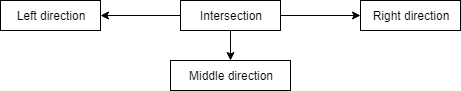
\includegraphics[width=400pt]{pic1.png}
	\caption{The eight maze possibilities}
	
\end{figure}
\begin{table}[h!]
	\begin{center}
		\begin{tabular}{||c c c |c||} 
			\hline
			Left & Middle & Right & State \\
			\hline\hline
			0 & 0 & 0 & Dead end \\ 
			\hline
			0 & 0 & 1 & Right only \\ 
			\hline
			0 & 1 & 0 & Straight only \\ 
			\hline
			0 & 1 & 1 & Straight or Right\\ 
			\hline
			1 & 0 & 0 & Left only \\ 
			\hline
			1 & 0 & 1 & Left of Right ("T" state)\\ 
			\hline
			1 & 1 & 0 & Straight or Left \\ 
			\hline
			1 & 1 & 1 & Four way \\ 
			\hline
		\end{tabular}
		\caption{The eight maze possibilities (1 is opened, 0 is closed by the wall)}
		\label{table:1}
	\end{center}

\end{table}
\subsection{Result}
The servo turns its shaft by 30 degrees every second until it reaches 180 degrees and then decreases the angle back to 0 degrees by the same step.

\subsection{Behaviors}
The robot, virtually all of the precious time, will be engaged within the coming behaviours:\\
1. Sticking to the route, looking for another intersection.\\
2. At an intersection, choosing what kind of intersection it is.\\
3. At an intersection, make a turn.\\
These steps continue looping again and again until the robot reach the end of the maze.\\
\begin{figure}[h!]
	\centering
	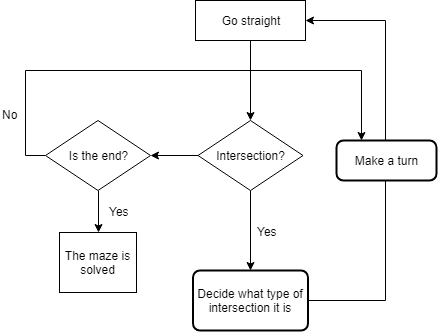
\includegraphics[width=400pt]{pic2.png}
	\caption{Behaviors}
\end{figure}

\subsection{The main algorithm}
• To be able to resolve the maze, the bot must traverse the maze two times.\\
• Within the very first run, it faces a little number of dead ends, but they are considered as "bad" paths; therefore, they can stay away from on the next run \cite{ref2}.\\
• The next is precisely how this particular algorithm works.\\
\subsubsection{Path stored in memory}
We use a 100-character string to store the path. The size could be more, but in this context, 100 is enough.
\subsubsection{Intersection and Turn Handling}
The robot has to be guided the appropriate action based on the kind of intersection or turn which it encounters.

\subsubsection{Mid and Right are open}
The bot senses a "Mid and Right" intersection. The left-hand rule is applied, then the robot goes straight.\\
The robot stays going straight and stores 'S' in memory.\\

\subsubsection{Dead-end}
In this particular situation, the bot has absolutely no option but to generate a 180-degree turn to exit the dead end. Since achieving a dead end implies that the bot has recently made a terrible turn, we have to keep the point; therefore, a prior turn is remedied. The BOE bot should not go to this particular dead end on the following run.\\
Path stored in memory will add character 'U' (because the dead-end shape is alike 'U' shape).

\subsubsection{Not intersection - Left only or Right only}
In these 2 cases, the bot has absolutely no option but generate a ninety-degree turn. Since the bot will invariably make the same ninety-degree turn and it is no other choice, this turn need never be saved when solving the maze.

\begin{lstlisting}[style=CStyle]
//irLeft, irMid or irRight equals to 1 when there is no wall, 0 otherwise
//Firstly, we defined that "state" value equals to (irLeft<<2) + (irRight<<1) + irMid
//We use bitwising to ease the way we read the state
//We use another function "translate()" to translate the state
//Eg. translate(1,1,0) = 6 i.e. Left and Right are open
if (state == leftOnly)
	turnLeft();
else if (state == rightOnly)
	turnRight();
\end{lstlisting}
\textit{\textbf{Reading states function:} Due to the inconsistency in reading the state of IR sensors, and the new function reading states will read the sensor value ten times in a matter of milliseconds then choose the state which shows up the most times.}
\begin{lstlisting}[style=CStyle]
int state() {
	//Array of counting state. Initially, all the values equal to 0
	d[8] = {0,0,0,0,0,0,0,0,0,0}; 
	Read IR 10 times {
		value equals to state of IR sensor;
		d[value] increases by 1;
		delay 10 milliseconds;
	}
	//maxd is the number of recurrence of the best state
	//res is the best state
	int maxd = -1, res = 0;
	for each state in 8 possibilities {
		if (maxd<d[state]) {
			update maxd = d[state]
			update res = state;
		}
	return res;
}
\end{lstlisting}

\subsubsection{Other types of intersection}
They are: Left and Mid, Left and Right, and three ways are open.\\
The left-hand rule requires a left turn, so take a character 'L' stored in the memory.

\subsubsection{Replacement Rules}
Every time after a character is stored in a memory; the algorithm will check three newest data to decide if the path could be reduced.\\
After every single turn, the length of the saved path increases by one. If the maze, for instance, features a long zigzag passageway with no side exits, a sequence like 'RLRLRLRL' shows up \cite{ref3}. There is simply no shortcut that could enable the robot to get through this area of the maze faster than simply after left hand on the wall structure technique. Nevertheless, every time it faces a dead end, it can streamline the path to something shorter.\\
Thinking about the sequence 'LUL', wherever U stands for a back, and it is the action taken when a dead end is encountered. This is what happens if there's a left turn that limbs off of a straight case and directs quickly to a dead end. After turning 90 degrees left, 180, and 90 degrees left again, and the total outcome would be that the bot is proceeding in its initial path again. The course could be made simple to a zero turn: one 'S' \cite{ref3}.\\
Another example is a \textit{T} intersection with a dead end on the left: 'LUS'. The turns are 90 degrees left, 180 degrees, and also 0 degrees, for a total of 90 degrees properly. The sequence must be replaced with a single 'R'.\\

In reality, each time the memory contains a sequence like 'xUx', we can change all three turns having a turn corresponding to the entire perspective, removing the U-turn and quickly change the solution. Here is the code to manage this:

\begin{lstlisting}[style=CStyle]
void simplify_path() {
	if(the length of memory < 2 || the second-to-last turn was a 'U')
		return;	
	int total_angle = 0;
	for each character of three last characters in the memory {
		in case 'R':
			total_angle increases by 90;
		in case 'L':
			total_angle increases by 270;
		in case 'U':
			total_angle increases by 180;
	}
	
	// Get the angle as a number between 0 and 360 degrees.
	total_angle = total_angle % 360;

	// Replace all of those turns with a single one.
	check total_angle {
		equals to 0:
			three last change in to 'S';
		equals to 90:
			three last change in to 'R';
		equals to 180:
			three last change in to 'U';
		equals to 270:
			three last change in to 'L';
	}
}
\end{lstlisting}

%section 5
\newpage
\section{Description of the prototype used for the demonstration}
\subsection{The system}
The diagram below shows the operation of the system after attaching Slave Bluetooth on the BOE robot and the Master one in a separate Arduino board controlled by the command typed by the user.\\
When we type the command "start" the robot will start at the beginning of the maze. Every second the robot moves, it sends the \textbf{state} to the master Bluetooth via slave Bluetooth. Then this status is continuously printed on the Serial output of Master Bluetooth.\\
The user needs to choose the end of the maze at everywhere of the maze. When the robot reaches the destination, the user has to send command "stop" to the robot then the robot will stop and finish collecting and simplifying the data in its memory. After that, the robot needs to be located at the beginning once again. At this stage, it will automatically find the shortest to solve the maze.\\  
\begin{figure}[h!]
	\centering
	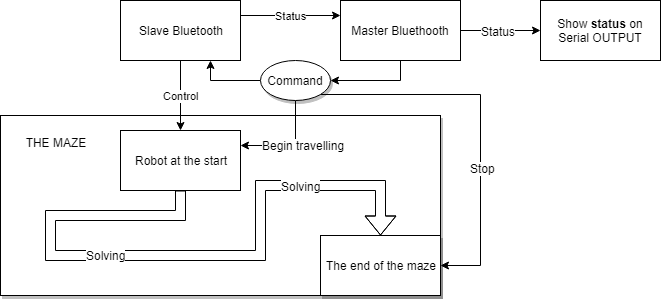
\includegraphics[width=500pt]{pic6.png}
	\caption{Operation of the system (sketched by Lucian)}
\end{figure}
\newpage
\subsection{Final product}
The following photos show the final assembly of the robot.\\
\begin{figure}[h!]
	\centering
	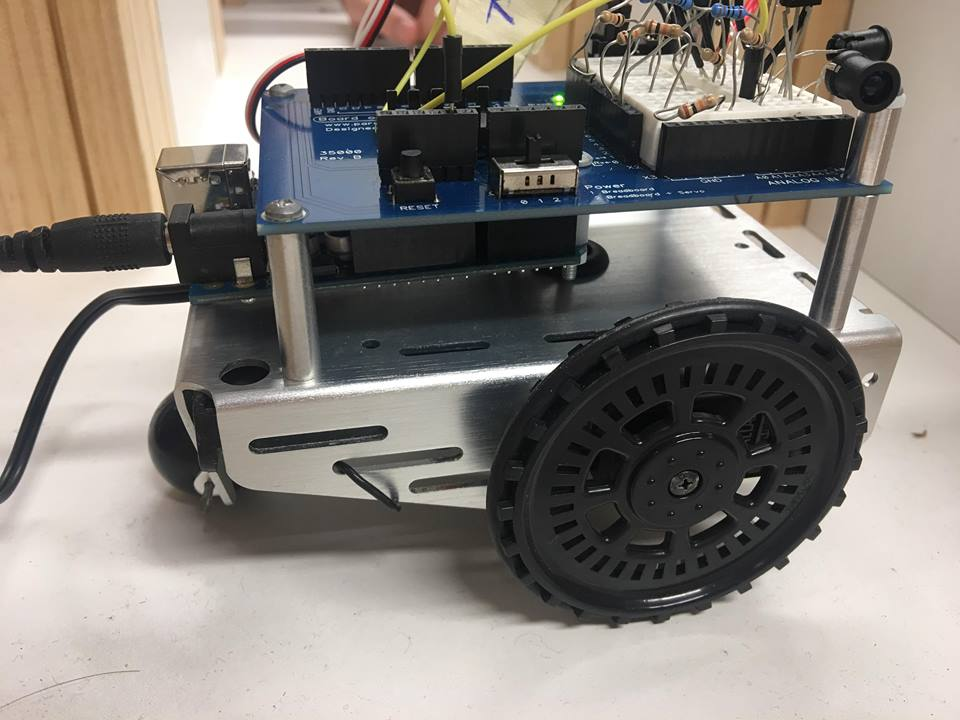
\includegraphics[width=400pt]{pic4.jpg}
	\caption{The maze solving robot}
\end{figure}
\begin{figure}[h!]
	\centering
	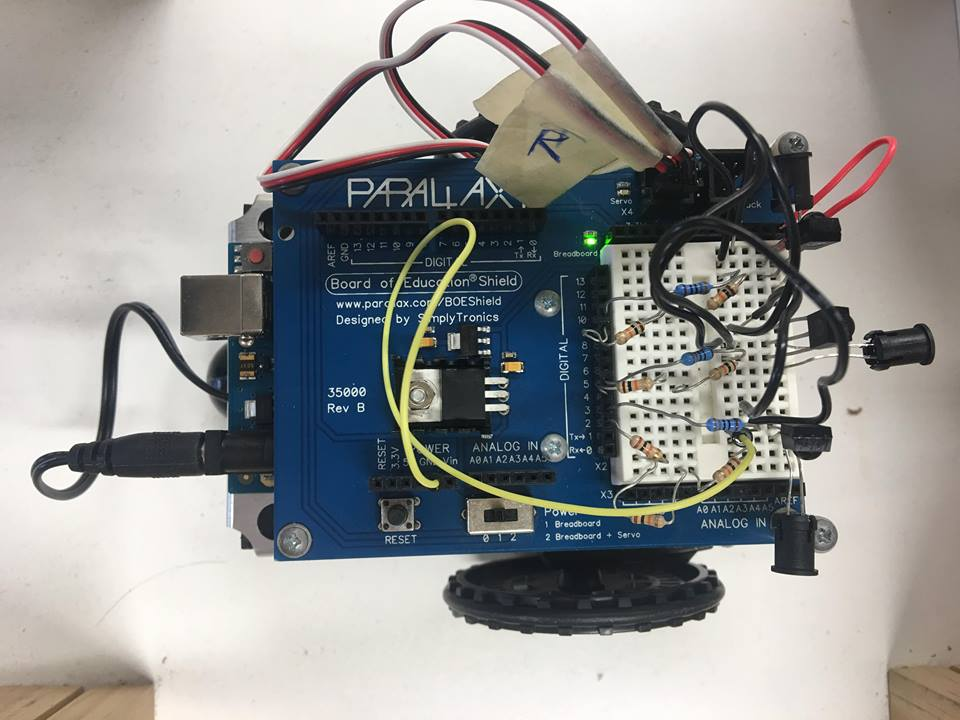
\includegraphics[width=400pt]{pic5.jpg}
	\caption{The maze solving robot}
\end{figure}
\textit{We have changed the normal jumper wires into the tougher ones, to reduces the error in running the robot}
\newpage
\subsection{Prototype}
We chose 110-ohm resistors for the IR sensors.\\
The resistors for the left and right LEDs have to be 4,000-ohms to assure the distance of detection in a range of 5-7 cm.\\
The resistor for the right LED has to be 6,000-ohm because the position of the LED is entirely convex compared to others.\\
\begin{figure}[h!]
	\centering
	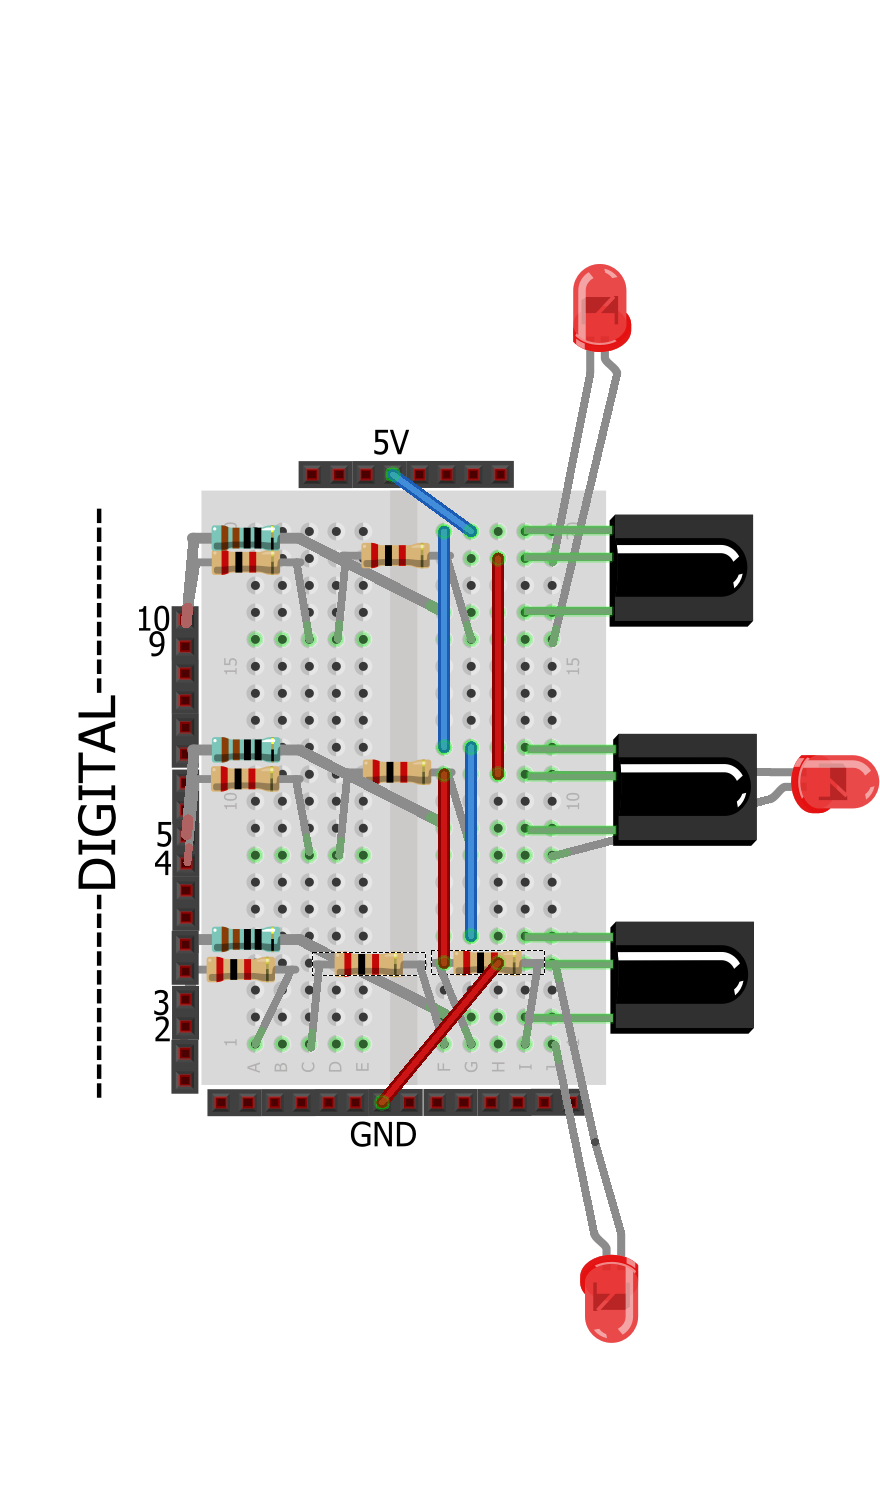
\includegraphics[width=400pt]{pic7.png}
	\caption{The sketch of Prototype (sketched by Keene)}
\end{figure}

\newpage
% Section 6
\section{Conclusion}
In conclusion, the objective of the project is to find a way out of the maze without impacting any objects. To accomplish our purpose, we implement the sensors to the robot so that it can detect the barriers on three sides. Besides that, we use a maze-solving algorithm to direct the robot from walls and get out of the maze. The result is found to meet our initial expectation. The robot successfully went through the maze and can detect walls. The crucial factor that contributes to our team success is the teamwork. Every team members complete their assignment correctly on time. In our team meeting, we propose problems that need to be solved and point out the right direction for the project.   However, the process of fulfilling the task is not smoothly perfect. For example, Arduino programming language appears distinctly different from other languages, the selection of resistors account for an enormous amount of time and so on but we manage to go through all those barriers. From the project, we all learn a brand-new language or how to implement the sensors to a real project which is possibly helpful for our course. Besides, we learn how to work together as a team and how to compensate for members' shortcomings.


% Section 7
\newpage
\section{Appendices}
\subsection{Code listing}
\textbf{\textit{SLAVE.ino}}
\begin{lstlisting}[style=CStyle]
#include <SoftwareSerial.h>   //Software Serial Port
#include <StackArray.h>
#include <Servo.h>

// https://www.pololu.com/file/0J195/line-maze-algorithm.pdf

Servo servoLeft;
Servo servoRight;
const int pinServoLeft = 13;
const int pinServoRight = 12;
const int pinLeftLED = 9 ;
const int pinRightLED = 2;
const int pinMidLED = 4;
const int pinLeftReceiver = 10;
const int pinRightReceiver = 3 ;
const int pinMidReceiver = 5;
const int frequency = 38000;
bool onTrace = false;
int cc = 0;
// StackArray <int> stack;
String mem="                                                                                                    ";
int memPointer=0;
#define RxD 7

#define TxD 6



#define DEBUG_ENABLED  1



SoftwareSerial blueToothSerial(RxD,TxD);

void moveForward() {
	servoLeft.attach(pinServoLeft);
	servoRight.attach(pinServoRight);
	servoLeft.writeMicroseconds(1700);
	servoRight.writeMicroseconds(1300);
	delay(1500);
	servoLeft.detach();                            // Stop servo signals
	servoRight.detach();
	delay(1000);
}

void reverse() {
	servoLeft.attach(pinServoLeft);
	servoRight.attach(pinServoRight);
	servoLeft.writeMicroseconds(1700);
	servoRight.writeMicroseconds(1700);
	delay(1000);
	servoLeft.detach();                            // Stop servo signals
	servoRight.detach();
	delay(1000);
}

void turnLeft() {
	servoLeft.attach(pinServoLeft);
	servoRight.attach(pinServoRight);
	servoLeft.writeMicroseconds(1300);
	servoRight.writeMicroseconds(1300);
	delay(450);
	servoLeft.detach();                            // Stop servo signals
	servoRight.detach();
	delay(1000);
}

void turnRight() {
	servoLeft.attach(pinServoLeft);
	servoRight.attach(pinServoRight);
	servoLeft.writeMicroseconds(1700);
	servoRight.writeMicroseconds(1700);
	delay(480);
	servoLeft.detach();                            // Stop servo signals
	servoRight.detach();
	delay(1000);
}

void hold() {
	servoLeft.attach(pinServoLeft);
	servoRight.attach(pinServoRight);
	servoLeft.writeMicroseconds(1500);
	servoRight.writeMicroseconds(1500);
	servoLeft.detach();                            // Stop servo signals
	servoRight.detach();
	delay(1000);
}

int irDetect(int irLedPin, int irReceiverPin, int frequency)
{
	tone(irLedPin, frequency, 8);              // IRLED 38 kHz for at least 1 ms
	delay(1);                                  // Wait 1 ms
	int ir = digitalRead(irReceiverPin);       // IR receiver -> ir variable
	delay(1);                                  // Down time before recheck
	return ir;                                // Return 1 no detect, 0 detect
}

int state() {
	int d[8] = {0,0,0,0,0,0,0,0};
	for(int i=0;i<10;++i) {
		int irLeft = irDetect(pinLeftLED, pinLeftReceiver, frequency);       // Check for object on left
		int irRight = irDetect(pinRightLED, pinRightReceiver, frequency);       // Check for object on right
		int irMid = irDetect(pinMidLED, pinMidReceiver, frequency);
		int value = irLeft * 4 + irRight * 2 + irMid;
		d[value] = d[value]+1;
		delay(10);
	}
	int maxd = -1,res=0;
	for(int i=0;i<8;++i)
		if(maxd<d[i]) {
			maxd=d[i];
			res=i;
		}

	return res;
}
int translate(int l, int r, int m) {
	return l * 4 + r * 2 + m;
}

void setup()
{

	Serial.begin(9600);
	pinMode(RxD, INPUT);
	pinMode(TxD, OUTPUT);
	setupBlueToothConnection();
	servoLeft.attach(pinServoLeft);
	servoRight.attach(pinServoRight);
	pinMode(pinLeftLED, OUTPUT);  pinMode(pinLeftReceiver, INPUT);
	pinMode(pinRightLED, OUTPUT);  pinMode(pinRightReceiver, INPUT);
	pinMode(pinMidLED, OUTPUT); pinMode(pinMidReceiver, INPUT);
	mem[memPointer]='s';

}

void simplify_path()
{
	// only simplify the path if the second-to-last turn was a 'u'
	if(memPointer < 2 || mem[memPointer-1] != 'u')
		return;

	int total_angle = 0;
	for(int i=1;i<=3;++i)
	{
		switch(mem[memPointer-i+1])
		{
			case 'r':
				total_angle += 90;
				break;
			case 'l':
			total_angle += 270;
			break;
			case 'u':
			total_angle += 180;
			break;
		}
	}

	// Get the angle as a number between 0 and 360 degrees.
	total_angle = total_angle % 360;
	
	// Replace all of those turns with a single one.
	switch(total_angle)
	{
		case 0:
			mem[memPointer - 2] = 's';
			break;
		case 90:
			mem[memPointer - 2] = 'r';
			break;
		case 180:
			mem[memPointer - 2] = 'u';
			break;
		case 270:
			mem[memPointer - 2] = 'l';
			break;
	}

	// The path is now two steps shorter.
	memPointer -= 2;
}



void lo1op()
{
	int cnt = 0;
	char cur;
	while(cnt<6) {
		if(blueToothSerial.available()) {
			cur = blueToothSerial.read();
			delay(1);
		}
	
		cnt += 1;
		delay(1);
	}
}

void loop() {
	// put your main code here, to run repeatedly:
	//  Serial.println(onReverse);
	//  delay(2000);
	char cur;
	int cnt = 0;
	while(cnt<6) {
		if(blueToothSerial.available()) {
			cur = blueToothSerial.read();
			delay(1);
		}
		if(cur == 'x') {
			if(!onTrace)
				onTrace = true;
			else
				onTrace = false;
			hold();
			break;
		}
		cnt += 1;
		delay(50);
	}
	while(true) {
		if(blueToothSerial.available()) {
			cur = blueToothSerial.read();
			delay(1);
		}
		if(cur == '`') {
			break;
		} else if(cur == '[') {
			servoLeft.attach(pinServoLeft);
			servoRight.attach(pinServoRight);
			servoLeft.writeMicroseconds(1300);
			servoRight.writeMicroseconds(1300);
			delay(25);
			servoLeft.detach();                            // Stop servo signals
			servoRight.detach();
		} else if (cur == ']') {
			servoLeft.attach(pinServoLeft);
			servoRight.attach(pinServoRight);
			servoLeft.writeMicroseconds(1700);
			servoRight.writeMicroseconds(1700);
			delay(25);
			servoLeft.detach();                            // Stop servo signals
			servoRight.detach();
		}
		delay(50);
	}
	
	if(onTrace==false) {
		int current = state();
		blueToothSerial.print(current);
		if (current == 1) {
			moveForward();
		} else if (current == 0) {
			reverse();
			moveForward();
			++memPointer;
			mem[memPointer]='u';
		} else {
			if (current == translate(1, 0, 0)) {
			turnLeft();
			moveForward();
		}
		else if (current == translate(0, 1, 0)) {
			turnRight();
			moveForward();
		}
		else if (current == translate(1, 0, 1)) {
			turnLeft();
			moveForward();
			++memPointer;
			mem[memPointer]='l';
		}
		else if (current ==  translate(0, 1, 1)) {
			moveForward();
			++memPointer;
			mem[memPointer]='s';
		} else if (current == translate(1, 1, 0)) {
			turnLeft();
			moveForward();
			++memPointer;
			mem[memPointer]='l';
		} else if (current == translate(1, 1, 1)) {
			turnLeft();
			moveForward();
			++memPointer;
			mem[memPointer]='l';
		}
	}
	simplify_path();
	} else {
		int current = state();
		if (current == 1) {
			moveForward();
		} else  if (current == translate(1, 0, 0)) {
			turnLeft();
			moveForward();
		} else if (current == translate(0, 1, 0)) {
			turnRight();
			moveForward();
		} else {
			if(mem[cc] == 's') {
				moveForward();
			} else if(mem[cc] == 'l') {
				turnLeft();
				moveForward();
			} else if(mem[cc] == 'r') {
				turnRight();
				moveForward();
			}
		}
	}

}



void setupBlueToothConnection()
{
	blueToothSerial.begin(38400);                           // Set BluetoothBee BaudRate to default baud rate 38400
	blueToothSerial.print("\r\n+STWMOD=0\r\n");             // set the bluetooth work in slave mode
	blueToothSerial.print("\r\n+STNA=Slave30+\r\n");    // set the bluetooth name as "SeeedBTSlave"
	blueToothSerial.print("\r\n+STOAUT=1\r\n");             // Permit Paired device to connect me
	blueToothSerial.print("\r\n+STAUTO=0\r\n");             // Auto-connection should be forbidden here
	delay(2000);                                            // This delay is required.
	blueToothSerial.print("\r\n+INQ=1\r\n");                // make the slave bluetooth inquirable
	Serial.println("The slave bluetooth is inquirable!");
	delay(2000);                                            // This delay is required.
	
	blueToothSerial.flush();

}


\end{lstlisting}

\textbf{\textit{MASTER.ino}}
\begin{lstlisting}[style=CStyle]
#include <SoftwareSerial.h>                     // Software Serial Port
#define RxD 7
#define TxD 6
#define DEBUG_ENABLED  1

String retSymb = "+RTINQ=";                     // start symble when there's any return
String slaveName = ";Slave30";             // caution that ';'must be included, and make sure the slave name is right.
int nameIndex = 0;
int addrIndex = 0;

String recvBuf;
String slaveAddr;
String connectCmd = "\r\n+CONN=";
SoftwareSerial blueToothSerial(RxD,TxD);



void setup()

{

	Serial.begin(9600);
	
	pinMode(RxD, INPUT);
	
	pinMode(TxD, OUTPUT);
	
	setupBlueToothConnection();
	
	//wait 1s and flush the serial buffer
	
	delay(1000);
	
	Serial.flush();
	
	blueToothSerial.flush();

}



void loop()

{
	
	char recvChar;
	
	while(1)
	
	{
	
		if(blueToothSerial.available())         //check if there's any data sent from the remote bluetooth shield
		
		{
	
			recvChar = blueToothSerial.read();
			switch(recvChar) {
				case '0': Serial.println("U-shape"); break;
				case '1': Serial.println("Straight only"); break;
				case '2': Serial.println("Right only"); break;
				case '3': Serial.println("Middle or Right"); break;
				case '4': Serial.println("Left only"); break;
				case '5': Serial.println("Middle or Left"); break;
				case '6': Serial.println("T-shape"); break;
				case '7': Serial.println("3-way shape"); break;
				case default: Serial.print(recvChar); break;
			}

		}

		if(Serial.available())                  //check if there's any data sent from the local serial terminal, you can add the other applications here
	
		{
	
			recvChar  = Serial.read();
			
			blueToothSerial.print(recvChar);
			
		}
	
	}
}



void setupBlueToothConnection()
{
		blueToothSerial.begin(38400);                               // Set BluetoothBee BaudRate to default baud rate 38400
		blueToothSerial.print("\r\n+STWMOD=1\r\n");                 // set the bluetooth work in master mode
		
		blueToothSerial.print("\r\n+STNA=Master11\r\n");       // set the bluetooth name as
		
		blueToothSerial.print("\r\n+STAUTO=0\r\n");                 // Auto-connection is forbidden here
		delay(2000);                                                // This delay is required.
		blueToothSerial.flush();
		blueToothSerial.print("\r\n+INQ=1\r\n");                    //make the master inquire
		Serial.println("Master is inquiring!");
		delay(2000); // This delay is required.
	
	
	
		//find the target slave
		
		char recvChar;

		while(1)
		
		{
		
			if(blueToothSerial.available())
			
			{
		
				recvChar = blueToothSerial.read();
				
				recvBuf += recvChar;
				
				nameIndex = recvBuf.indexOf(slaveName);             //get the position of slave name
		
		
		
				//nameIndex -= 1;
			
				//decrease the ';' in front of the slave name, to get the position of the end of the slave address
			
				if ( nameIndex != -1 )
			
				{
		
					//Serial.print(recvBuf);
		
					addrIndex = (recvBuf.indexOf(retSymb,(nameIndex - retSymb.length()- 18) ) + retSymb.length());//get the start position of slave address
					
					slaveAddr = recvBuf.substring(addrIndex, nameIndex);//get the string of slave address
					
					break;

				}

			}

		}



		//form the full connection command
		
		connectCmd += slaveAddr;
		
		connectCmd += "\r\n";
		
		int connectOK = 0;
		
		Serial.print("Connecting to slave:");
		
		Serial.print(slaveAddr);
		
		Serial.println(slaveName);
		
		//connecting the slave till they are connected

		do
		
		{
			
			blueToothSerial.print(connectCmd);//send connection command
			
			recvBuf = "";

			while(1)
			
			{
				
				if(blueToothSerial.available()){
				
				recvChar = blueToothSerial.read();
				
				recvBuf += recvChar;

				if(recvBuf.indexOf("CONNECT:OK") != -1)
				
				{
					
					connectOK = 1;
					
					Serial.println("Connected!");
					
					blueToothSerial.print("Connected!");
					
					break;
				
				}

				else if(recvBuf.indexOf("CONNECT:FAIL") != -1)
				
				{

					Serial.println("Connect again!");

					break;

				}

			}

		}

	}while(0 == connectOK);

}

\end{lstlisting}


\subsection{Link to Trello Board}
\href{https://trello.com/b/9y4uQUCG/project}{\textit{Link to Trello Board of the team.}}
%----------------------------------------------------------------------------------------

%----------------------------------------------------------------------------------------

\newpage
\bibliographystyle{IEEEtranN}
\bibliography{project}
\end{document}